%%%%%%%%%%%%%%%%%%%%%%%%%%%%%%%%%%%%%%%%%
% Beamer Presentation
% LaTeX Template
% Version 1.0 (10/11/12)
%
% This template has been downloaded from:
% http://www.LaTeXTemplates.com
%
% License:
% CC BY-NC-SA 3.0 (http://creativecommons.org/licenses/by-nc-sa/3.0/)
%
%%%%%%%%%%%%%%%%%%%%%%%%%%%%%%%%%%%%%%%%%

%----------------------------------------------------------------------------------------
%	PACKAGES AND THEMES
%----------------------------------------------------------------------------------------

\documentclass{beamer}
%\usepackage{listings}
\mode<presentation> {

% The Beamer class comes with a number of default slide themes
% which change the colors and layouts of slides. Below this is a list
% of all the themes, uncomment each in turn to see what they look like.

%\usetheme{default}
%\usetheme{AnnArbor}
%\usetheme{Antibes}
%\usetheme{Bergen}
%\usetheme{Berkeley}
%\usetheme{Berlin}
%\usetheme{Boadilla}
%\usetheme{CambridgeUS}
%\usetheme{Copenhagen}
%\usetheme{Darmstadt}
%\usetheme{Dresden}
%\usetheme{Frankfurt}
%\usetheme{Goettingen}
%\usetheme{Hannover}
%\usetheme{Ilmenau}
%\usetheme{JuanLesPins}
%\usetheme{Luebeck}
\usetheme{Madrid}
%\usetheme{Malmoe}
%\usetheme{Marburg}
%\usetheme{Montpellier}
%\usetheme{PaloAlto}
%\usetheme{Pittsburgh}
%\usetheme{Rochester}
%\usetheme{Singapore}
%\usetheme{Szeged}
%\usetheme{Warsaw}

% As well as themes, the Beamer class has a number of color themes
% for any slide theme. Uncomment each of these in turn to see how it
% changes the colors of your current slide theme.

%\usecolortheme{albatross}
%\usecolortheme{beaver}
%\usecolortheme{beetle}
%\usecolortheme{crane}
%\usecolortheme{dolphin}
%\usecolortheme{dove}
%\usecolortheme{fly}
%\usecolortheme{lily}
%\usecolortheme{orchid}
%\usecolortheme{rose}
%\usecolortheme{seagull}
%\usecolortheme{seahorse}
%\usecolortheme{whale}
%\usecolortheme{wolverine}

%\setbeamertemplate{footline} % To remove the footer line in all slides uncomment this line
%\setbeamertemplate{footline}[page number] % To replace the footer line in all slides with a simple slide count uncomment this line

%\setbeamertemplate{navigation symbols}{} % To remove the navigation symbols from the bottom of all slides uncomment this line
}
\usepackage{listings}
\usepackage{graphicx} % Allows including images
\usepackage{booktabs} % Allows the use of \toprule, \midrule and \bottomrule in tables
\usepackage{animate}

%----------------------------------------------------------------------------------------
%	TITLE PAGE
%----------------------------------------------------------------------------------------

\title[Halo exchange on BG/Q]{Modeling halo exchange on the BlueGene/Q} % The short title appears at the bottom of every slide, the full title is only on the title page

\author{Yadu N. Babuji \& Tim Armstrong} % Your name
\institute[Dept. of Computer Science]
{
The University of Chicago \\
\medskip
}
\date{\today} % Date, can be changed to a custom date

\begin{document}

\begin{frame}
\titlepage % Print the title page as the first slide
\end{frame}

\begin{frame}
\frametitle{Overview} % Table of contents slide, comment this block out to remove it
\tableofcontents % Throughout your presentation, if you choose to use \section{} and \subsection{} commands, these will automatically be printed on this slide as an overview of your presentation
\end{frame}

%----------------------------------------------------------------------------------------
%	PRESENTATION SLIDES
%----------------------------------------------------------------------------------------

%------------------------------------------------
\section{Halo Exchange - Intro} % Sections can be created in order to organize your presentation into discrete blocks, all sections and subsections are automatically printed in the table of contents as an overview of the talk

%------------------------------------------------
\begin{frame}
\frametitle{Domain decomposition in parallel applications}
\begin{itemize}
  \item Parallelizing an application requires
      \emph{decomposing} the problem into multiple subproblems
      that are assigned to processors
  \item \emph{Domain decomposition} decomposes based on the application
          domain, e.g. spatially or temporally
\end{itemize}
\vspace{-1.0em}
\begin{figure}
  \centering
  \caption{Hurricane simulation using WRF software}
    %\animategraphics[loop,autoplay,width=0.45\linewidth]{12}{img/Typhoon_Mawar_2005_computer_simulation-frame}{0}{48}
    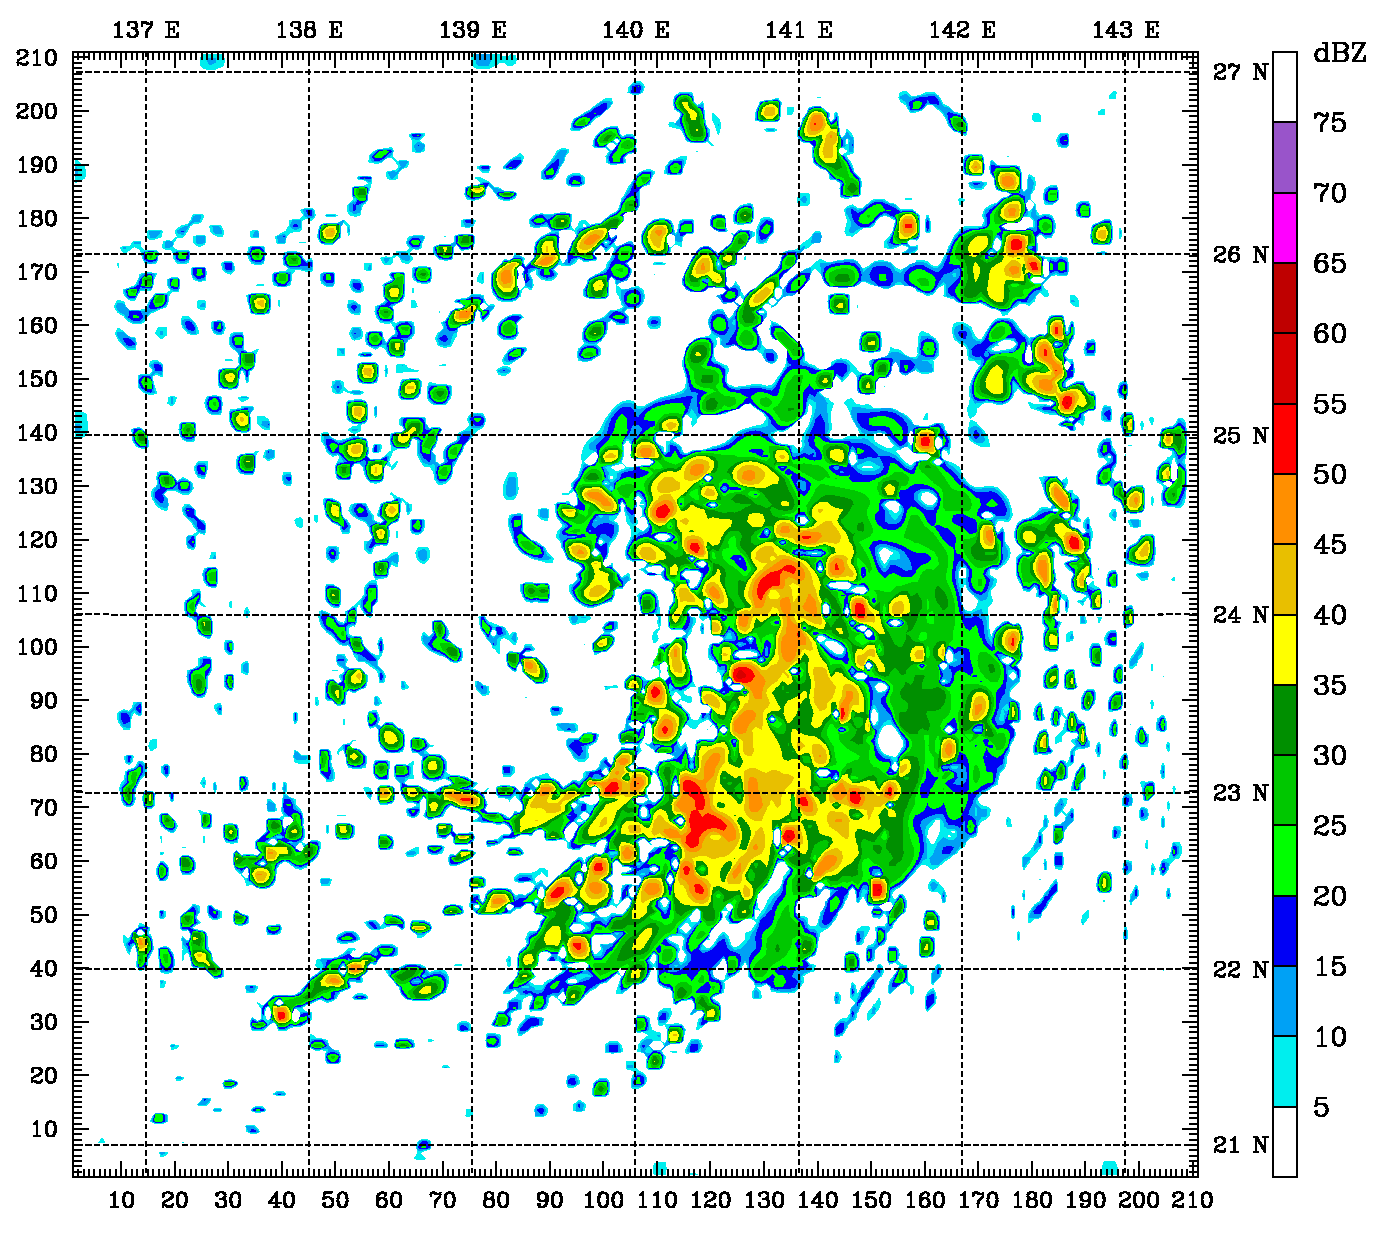
\includegraphics[width=0.45\linewidth]{img/Typhoon_Mawar_2005_computer_simulation-frame24}

\end{figure}
\end{frame}
%------------------------------------------------

%------------------------------------------------
\begin{frame}
\frametitle{Halo Exchange}
\begin{itemize}
  \item Halo exchange is a common nearest neighbor communication pattern
        associated with domain decomposition
  \item Boundary regions are periodically communicated to neighbors
\end{itemize}
\begin{figure}
  \centering
  \caption{Halo exchange for a 2D cartesian domain with wraparound on 8 processors}
  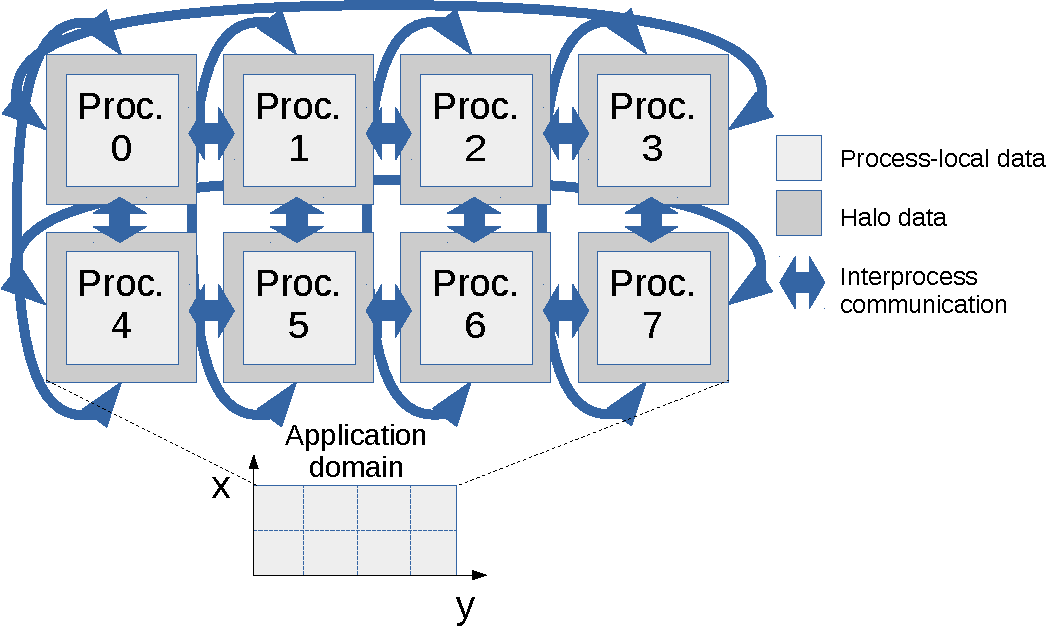
\includegraphics[width=0.55\linewidth]{../fig/halo-illustration}
\end{figure}
\end{frame}
%------------------------------------------------

%------------------------------------------------
\begin{frame}
\frametitle{Blue Gene/Q Mira}
\begin{itemize}
\item Argonne National Laboratory's flagship supercomputer
\item 48 racks, 49,152 nodes, 786,432 cores
\item 5-dimensional torus network
  \begin{itemize}
    \item Max 3$\mu$s latency, typically less
    \item Each node has (A, B, C, D, E) coordinates
    \item 10 network links to neighbours per node
    \item Messages for non-neighbours routed via multiple links
    \item 1.8 GB/s usable bandwidth per direction per link
  \end{itemize}
\end{itemize}
\vspace{-1.0em}
\centering
\begin{figure}
  \begin{minipage}{0.45\textwidth}
    \centering
    \caption{Blue Gene/Q Mira}
    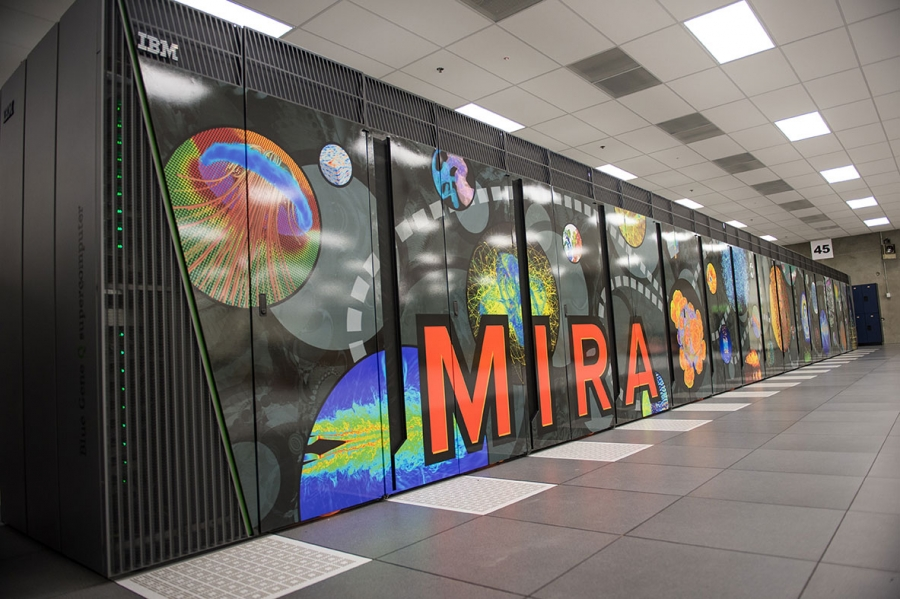
\includegraphics[width=0.9\linewidth]{mira}
  \end{minipage}
  \begin{minipage}{0.45\textwidth}
    \centering
    \caption{3-dimensional torus network for illustration}
    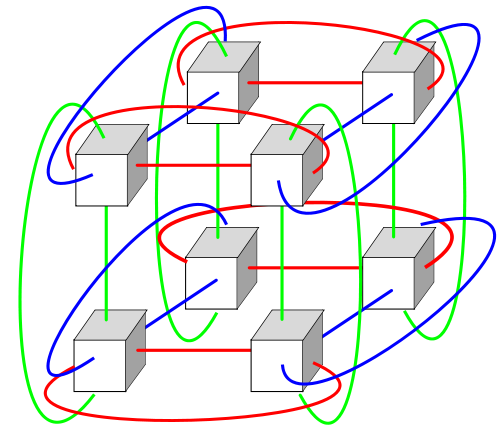
\includegraphics[width=0.65\linewidth]{500px-2x2x2torus}
  \end{minipage}
\end{figure}
\end{frame}
%------------------------------------------------

%------------------------------------------------
\begin{frame}
\frametitle{Task placement in Halo exchange}
\begin{itemize}
\item Problem setup:
  \begin{itemize}
    \item Application domain decomposed with cartesian grid, e.g. 32x32x8
    \item Network topology - 5D torus, e.g. 4x4x4x4x2 nodes, 16 cores/node
    \item Task mapping from application rank to network coordinate
  \end{itemize}
\item Easy optimization - no algorithmic or code changes required
\item Up to 7.5x difference in halo exchange time between mappings
\end{itemize}
\vspace{-1.0em}
\begin{figure}
  \centering
%  \caption{Task mapping for halo exchange}
  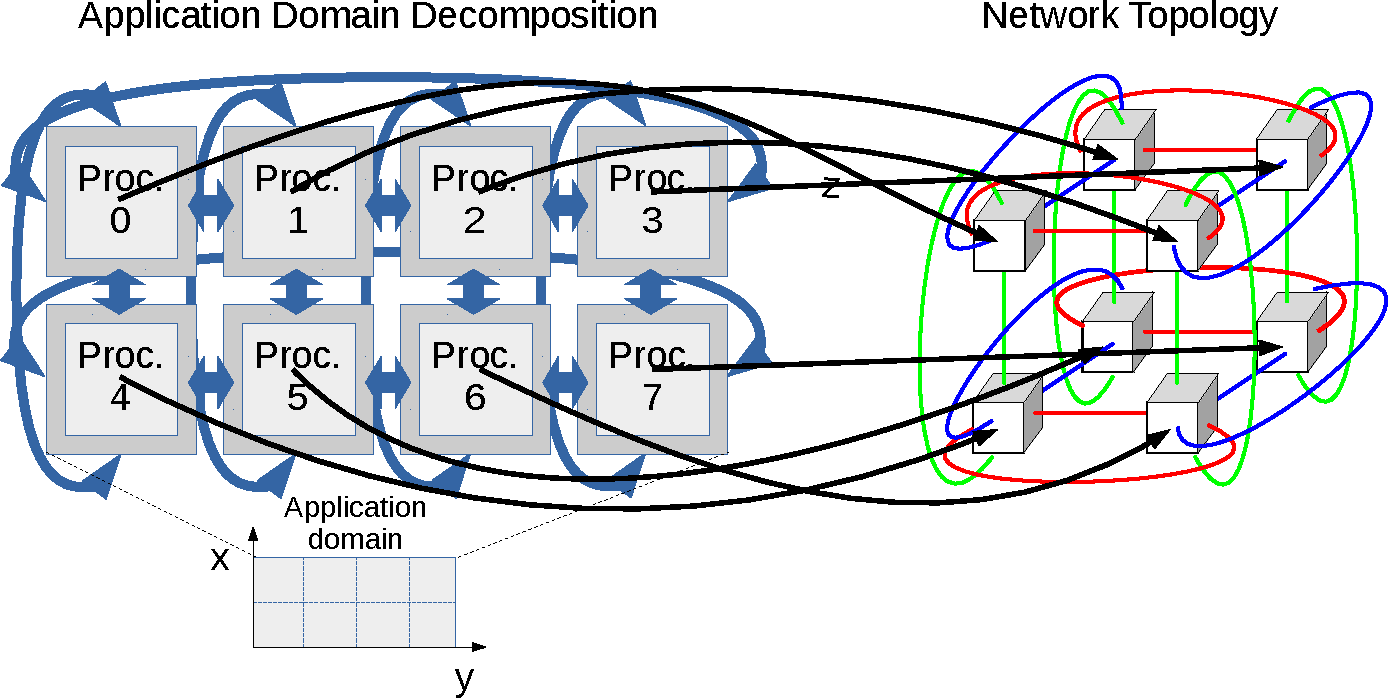
\includegraphics[width=0.75\linewidth]{../fig/halo-mapping}
\end{figure}
\end{frame}
%------------------------------------------------

%------------------------------------------------
\section{Contributions}
\begin{frame}[fragile]
\frametitle{Goals}
\begin{itemize}
  \item Predict task mapping performance for halo exchange on Blue Gene/Q
  \begin{itemize}
    \item Map application rank to (A, B, C, D, E, T) network coordinates
  \end{itemize}
  \item Discover good (and bad) task mapping strategies
\end{itemize}
\begin{figure}
  \centering
  \caption{Blue Gene/Q mapping file sample}
  \begin{lstlisting}[basicstyle=\footnotesize\ttfamily, frame=lines,columns=fixed]
A B C D E T
0 0 0 0 0 0
0 0 0 0 0 1
    ...
0 0 0 0 0 15
0 0 0 0 1 0
0 0 0 0 1 1
    ...
0 0 0 0 1 15
0 0 0 1 1 0
    ...
0 0 0 1 1 15
  \end{lstlisting}
\end{figure}
\end{frame}
%------------------------------------------------

%------------------------------------------------
\begin{frame}
\frametitle{What did we do?}
\begin{itemize}
\item We made an Analytical model from first principles to model the performance.
\item Introduced a reasonably effective metric for mappings
\item Experiments to study what factors affect performance
\item Made nearly optimal and pessimal mappings
\item Analysis and Plots!
\end{itemize}
\end{frame}
%------------------------------------------------

%------------------------------------------------
\section{Experiments}
\begin{frame}
\frametitle{Experiment Setup}
\begin{itemize}
  \item 512 node partition of Blue Gene/Q Mira at Argonne - 4x4x4x4x2
  \item 3D (32x32x8) and 5D (8x8x8x8x2) application domains with wraparound
  \item Message sizes from 8 bytes to 16MB
  \item Measured time for 6/10 concurrent sends and receives for 3D/5D
\end{itemize}

\centering
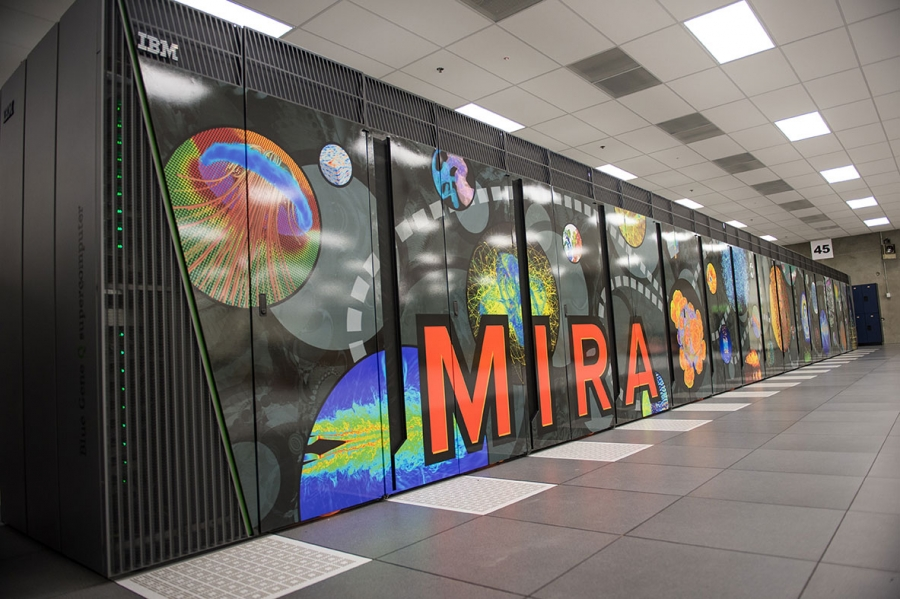
\includegraphics[width=0.45\linewidth]{mira}

\end{frame}
%------------------------------------------------

%------------------------------------------------
\begin{frame}
\frametitle{Impact of Message Size on Performance}
\begin{itemize}
  \item Some hypotheses we evaluated:
  \begin{itemize}
    \item Longer distances resulting in higher latency?
    \item Caching effects when message buffers do not fit in L3 cache?
    \item Different network protocols/routing algorithms
    \item Network congestion from increased traffic limits performance?
  \end{itemize}
\end{itemize}

\begin{figure}
TODO: basic time vs. data size plot
\end{figure}
\end{frame}

%------------------------------------------------

%================================================
\section{Experiment Plots}
%------------------------------------------------
\begin{frame}
\frametitle{Maximum distance and latency experiment}
\begin{itemize}
    \item Move one rank to furthest point in network from neighbor
    \item Do longer distances result in higher latency? Surprisingly, no!
\end{itemize}
\begin{figure}
%\caption{Latency effects}
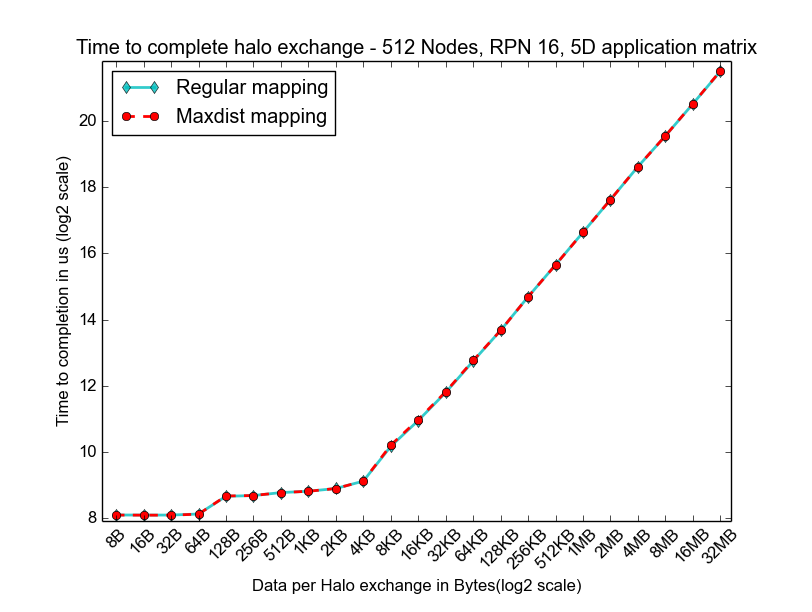
\includegraphics[width=0.8\linewidth]{../regular_vs_maxdist.png}
\end{figure}
\end{frame}
%------------------------------------------------

%------------------------------------------------
\begin{frame}
\frametitle{Caching effect experiments}
\begin{itemize}
    \item Caching effects when message buffers do not fit in L3 cache? No!
\end{itemize}
\begin{figure}
%\caption{Caching effects}
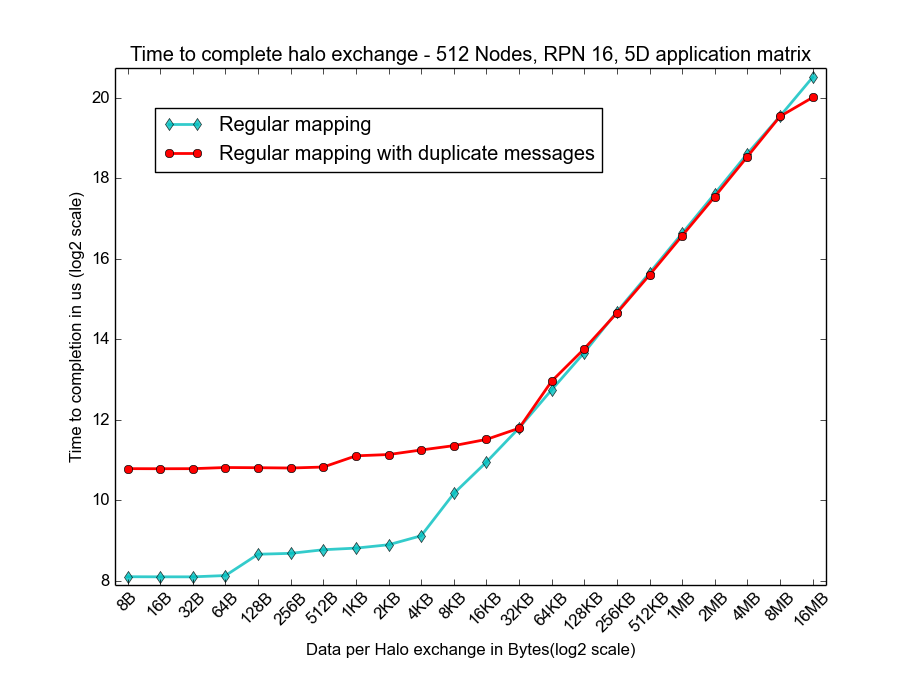
\includegraphics[width=0.8\linewidth]{../cache_duplicates_vs_regular.png}
\end{figure}
\end{frame}
%------------------------------------------------

%------------------------------------------------
\begin{frame}[fragile]
\frametitle{Blue Gene/Q Network protocols}
\begin{itemize}
    \item MPI protocol threshold values match experimental data
\end{itemize}
\begin{table}
  \caption{MPI Protocol default thresholds
    \label{table:bgq_protocols}}
  {\footnotesize
    \begin{tabular}{ | l | l | l | p{1.5cm} |}
    \hline 
    \input ../tables/protocols.tex
    \end{tabular}
  }
\end{table}
\end{frame}
%------------------------------------------------

%================================================
%------------------------------------------------
\section{Performance models}
\begin{frame}
\frametitle{Analytical model for Halo exchange performance}
\begin{itemize}
\item Total number of neighbors $T_{neighbors}$, D dimensionality of application.
\begin{equation}
  T_{neighbors} = N_{ranks} * 2 * D
\end{equation} \\
\item Average steps a message travels $N_{steps}$
\begin{equation}
  N_{steps} = \frac{ \sum\limits_{u,v} dist_{u,v} } {T_{neighbors}}
\end{equation} \\
\item Time to complete a halo exchange T with N bytes per message
\begin{equation}
  T = t_c + (N_{steps} * N_{procs} * N * t_b * \alpha)
\end{equation}
\item Model parameters:
\begin{itemize}
  \item $t_c$: constant start-up time
  \item $t_b$: time to transmit byte given ideal link utilization
  \item $\alpha$: link utilization factor
\end{itemize}
%\item $t_c$, and $\alpha$ are calibrated from experimental data. t_b is calculated from machine specifications.
\end{itemize}
\end{frame}
%------------------------------------------------

%------------------------------------------------
\section{Mappings}
\begin{frame}
\frametitle{What mapping strategies did we try?}
\begin{itemize}
\item Regular/Default
\item Skewed regular \& Skewed reversed
\item Random
\item Linear \& Reversed
\item \textbf{Pessimal mapping generated by Simulated Annealing}
\item \textbf{Optimal mapping by partitioning Application domains}
\end{itemize}
\end{frame}
%------------------------------------------------


%================================================
\section{Plots of Analytical Model and Experimental Data}

%------------------------------------------------
\begin{frame}
\frametitle{Overall traffic plots}
\begin{figure}
%\caption{Increasing traffic}
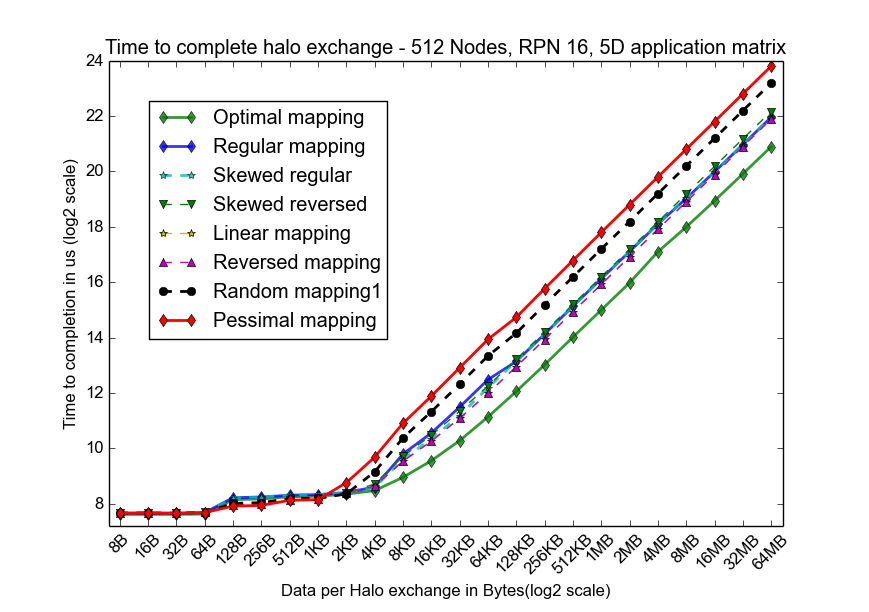
\includegraphics[width=0.8\linewidth]{../3D_512_all_mappings.png}
\end{figure}
\end{frame}
%------------------------------------------------

%------------------------------------------------
\begin{frame}[fragile]
\begin{figure}
\caption{5D Regular mapping}
\begin{columns}
  \begin{column}{0.6\textwidth}
    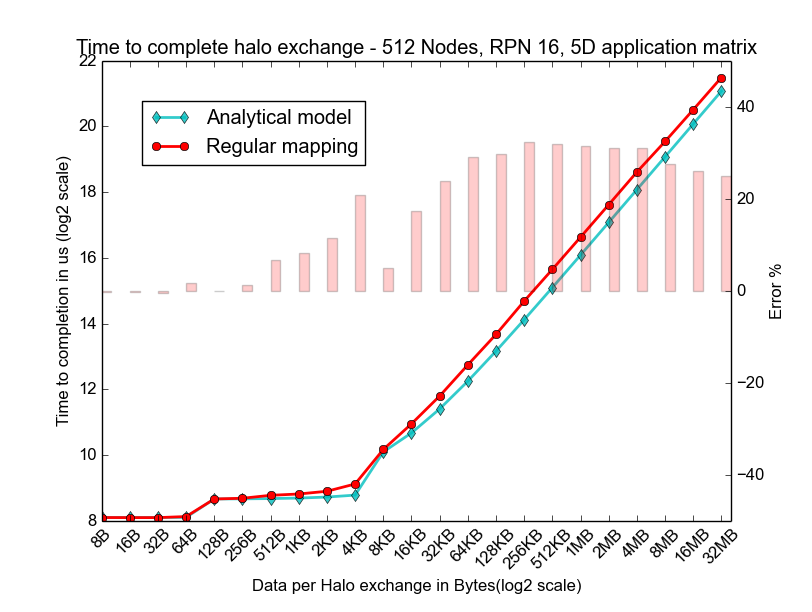
\includegraphics[width=1\textwidth]{../mappings/5d_regular_model.png}
  \end{column}
  \begin{column}{0.3\textwidth}
\lstset{title=Mapping sample}
\begin{lstlisting}[basicstyle=\footnotesize\ttfamily, frame=lines,columns=fixed]
0 0 0 0 0 0
    ...
0 0 0 0 0 15
0 0 0 0 1 0
    ...
0 0 0 0 1 15
0 0 0 1 1 0
    ...
0 0 0 1 1 15
\end{lstlisting}
  \end{column}
\end{columns}
\end{figure}
\end{frame}
%------------------------------------------------

%------------------------------------------------
\begin{frame}[fragile]
\begin{figure}
\caption{5D Linear mapping}
\begin{columns}
  \begin{column}{0.6\textwidth}
    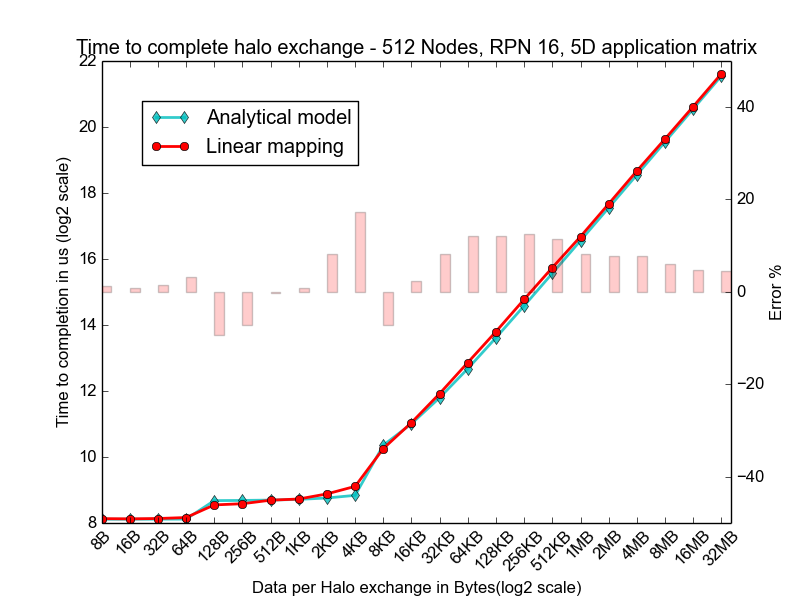
\includegraphics[width=1\textwidth]{../mappings/5d_linear_model.png}
  \end{column}
  \begin{column}{0.3\textwidth}
\lstset{title=Mapping sample}
\begin{lstlisting}[basicstyle=\footnotesize\ttfamily, frame=lines,columns=fixed]
0 0 0 0 0 0
1 0 0 0 0 0
2 0 0 0 0 0
3 0 0 0 0 0
0 1 0 0 0 0
1 1 0 0 0 0
2 1 0 0 0 0
3 1 0 0 0 0
0 2 0 0 0 0
\end{lstlisting}
  \end{column}

\end{columns}
\end{figure}
\end{frame}
%------------------------------------------------

%------------------------------------------------
\begin{frame}[fragile]
\begin{figure}
\caption{5D Skewed Regular}
\begin{columns}
  \begin{column}{0.6\textwidth}
    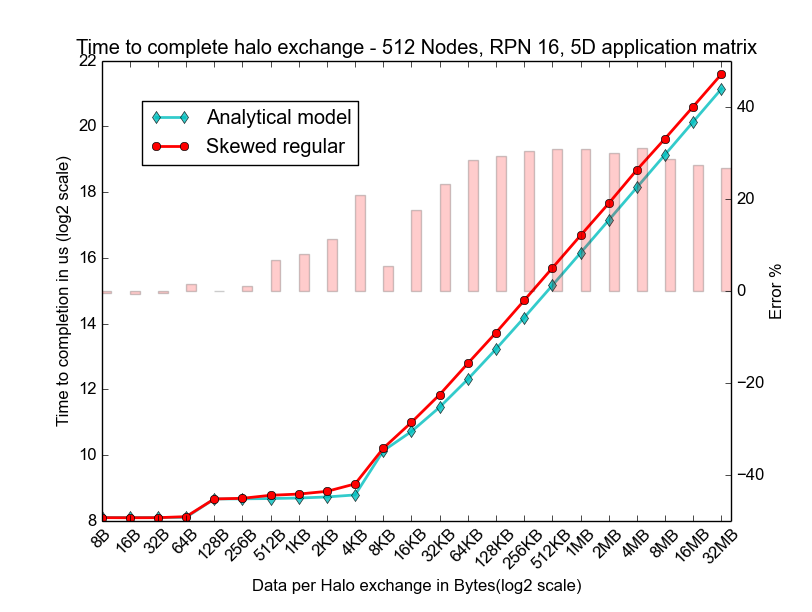
\includegraphics[width=1\textwidth]{../mappings/5d_skewed_regular.png}
  \end{column}
  \begin{column}{0.3\textwidth}
\lstset{title=Mapping sample}
\begin{lstlisting}[basicstyle=\footnotesize\ttfamily, frame=lines,columns=fixed]
0 0 0 0 0 0
  ...
0 0 0 0 0 15
0 0 0 0 1 0
  ...
0 0 0 0 1 15
0 0 0 2 0 0
  ...
0 0 0 2 0 15
\end{lstlisting}
  \end{column}
\end{columns}
\end{figure}
\end{frame}
%------------------------------------------------

%------------------------------------------------
\begin{frame}[fragile]
\begin{figure}
\caption{5D Skewed Reversed}
\begin{columns}
  \begin{column}{0.6\textwidth}
    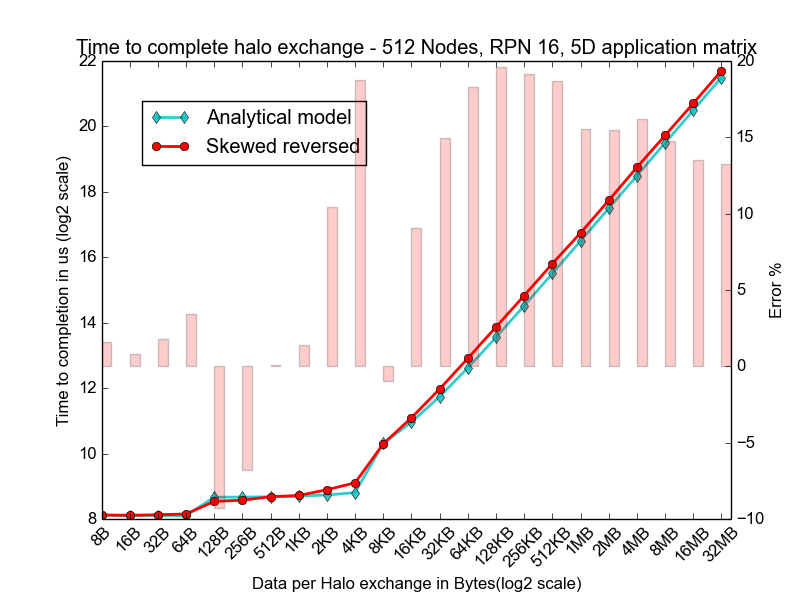
\includegraphics[width=1\textwidth]{../mappings/5d_skewed_reversed.png}
  \end{column}
  \begin{column}{0.3\textwidth}
\lstset{title=Mapping sample}
\begin{lstlisting}[basicstyle=\footnotesize\ttfamily, frame=lines,columns=fixed]
0 0 0 0 0 0
2 0 0 0 0 0
1 0 0 0 0 0
3 0 0 0 0 0
0 2 0 0 0 0
2 2 0 0 0 0
1 2 0 0 0 0
3 2 0 0 0 0
\end{lstlisting}
  \end{column}
\end{columns}
\end{figure}
\end{frame}
%------------------------------------------------

%------------------------------------------------
\begin{frame}
\begin{figure}
\caption{5D Random mapping}
    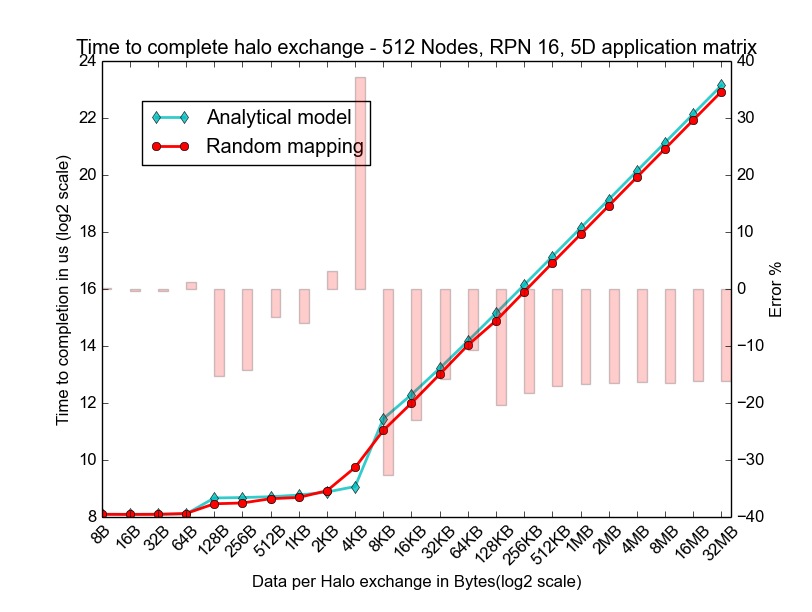
\includegraphics[width=0.75\textwidth]{../mappings/5d_random_model.png}
\end{figure}
\end{frame}
%------------------------------------------------

%------------------------------------------------
\begin{frame}[fragile]
\begin{figure}
\caption{5D Optimal mapping}
\begin{columns}
  \begin{column}{0.6\textwidth}
    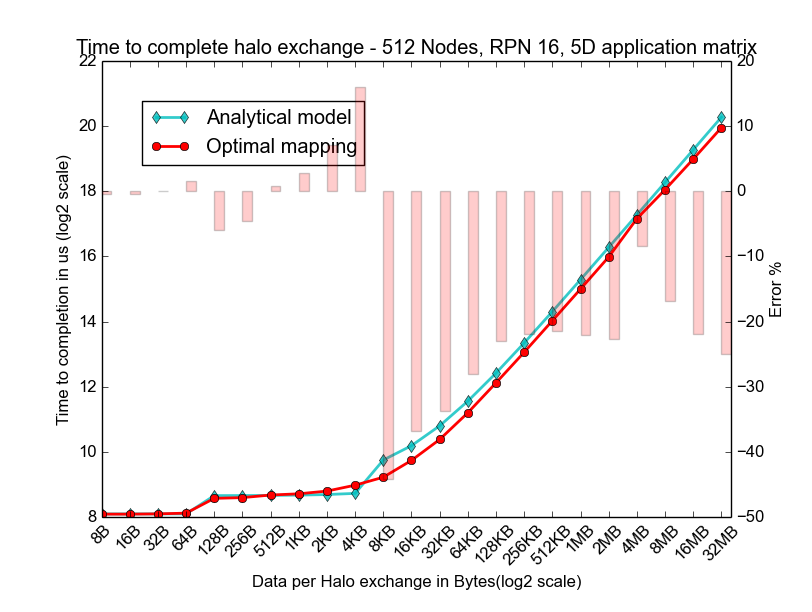
\includegraphics[width=1\textwidth]{../mappings/5d_optimal_model.png}
  \end{column}
  \begin{column}{0.3\textwidth}
\lstset{title=Mapping sample}
\begin{lstlisting}[basicstyle=\footnotesize\ttfamily, frame=lines,columns=fixed]
0 0 0 0 0 0
0 0 0 0 1 0
0 0 0 0 0 1
0 0 0 0 1 1
0 0 0 1 0 0
0 0 0 1 1 0
0 0 0 1 0 1
0 0 0 1 1 1
\end{lstlisting}
  \end{column}
\end{columns}
\end{figure}
\end{frame}
%------------------------------------------------


%------------------------------------------------
\begin{frame}[fragile]
\begin{figure}
\caption{3D Regular mapping}
\begin{columns}
  \begin{column}{0.6\textwidth}
    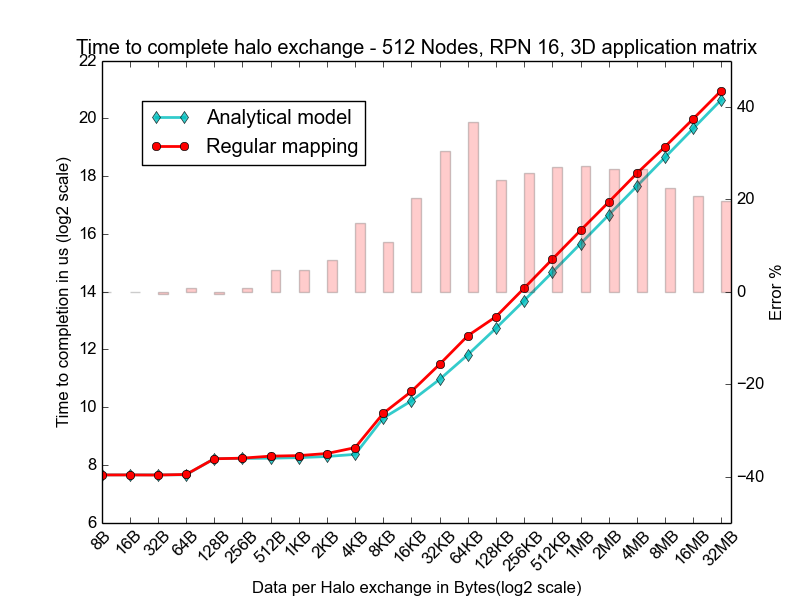
\includegraphics[width=1\textwidth]{../mappings/3d_regular.png}
  \end{column}
  \begin{column}{0.3\textwidth}
\lstset{title=Mapping sample}
\begin{lstlisting}[basicstyle=\footnotesize\ttfamily, frame=lines,columns=fixed]
0 0 0 0 0 0
    ...
0 0 0 0 0 15
0 0 0 0 1 0
    ...
0 0 0 0 1 15
0 0 0 1 1 0
    ...
0 0 0 1 1 15
\end{lstlisting}
  \end{column}
\end{columns}
\end{figure}
\end{frame}
%------------------------------------------------

%------------------------------------------------
\begin{frame}[fragile]
\begin{figure}
\caption{3D Linear mapping}
\begin{columns}
  \begin{column}{0.6\textwidth}
    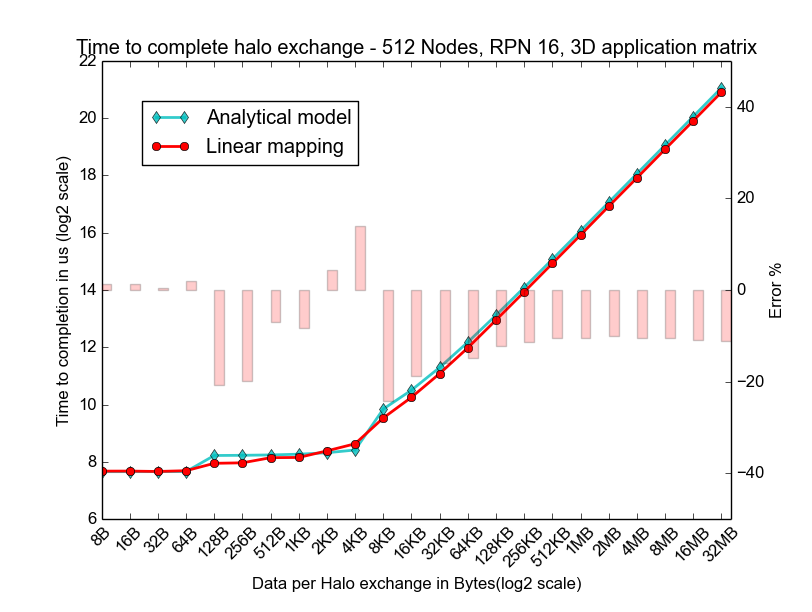
\includegraphics[width=1\textwidth]{../mappings/3d_linear.png}
  \end{column}
  \begin{column}{0.3\textwidth}
\lstset{title=Mapping sample}
\begin{lstlisting}[basicstyle=\footnotesize\ttfamily, frame=lines,columns=fixed]
0 0 0 0 0 0
1 0 0 0 0 0
2 0 0 0 0 0
3 0 0 0 0 0
0 1 0 0 0 0
1 1 0 0 0 0
2 1 0 0 0 0
3 1 0 0 0 0
0 2 0 0 0 0
\end{lstlisting}
  \end{column}

\end{columns}
\end{figure}
\end{frame}
%------------------------------------------------

%------------------------------------------------
\begin{frame}[fragile]
\begin{figure}
\caption{3D Skewed Regular}
\begin{columns}
  \begin{column}{0.6\textwidth}
    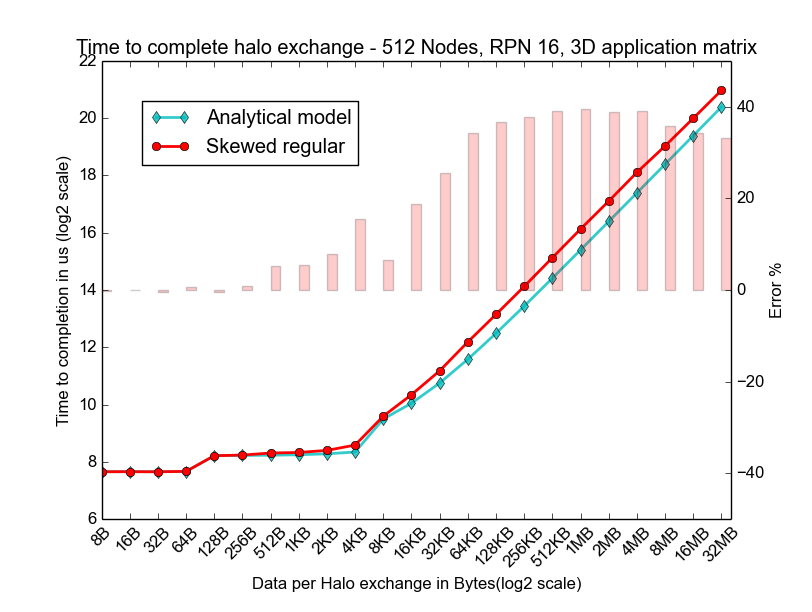
\includegraphics[width=1\textwidth]{../mappings/3d_skewed_regular.png}
  \end{column}
  \begin{column}{0.3\textwidth}
\lstset{title=Mapping sample}
\begin{lstlisting}[basicstyle=\footnotesize\ttfamily, frame=lines,columns=fixed]
0 0 0 0 0 0
  ...
0 0 0 0 0 15
0 0 0 0 1 0
  ...
0 0 0 0 1 15
0 0 0 2 0 0
  ...
0 0 0 2 0 15
\end{lstlisting}
  \end{column}
\end{columns}
\end{figure}
\end{frame}
%------------------------------------------------

%------------------------------------------------
\begin{frame}[fragile]
\begin{figure}
\caption{3D Skewed Reversed}
\begin{columns}
  \begin{column}{0.6\textwidth}
    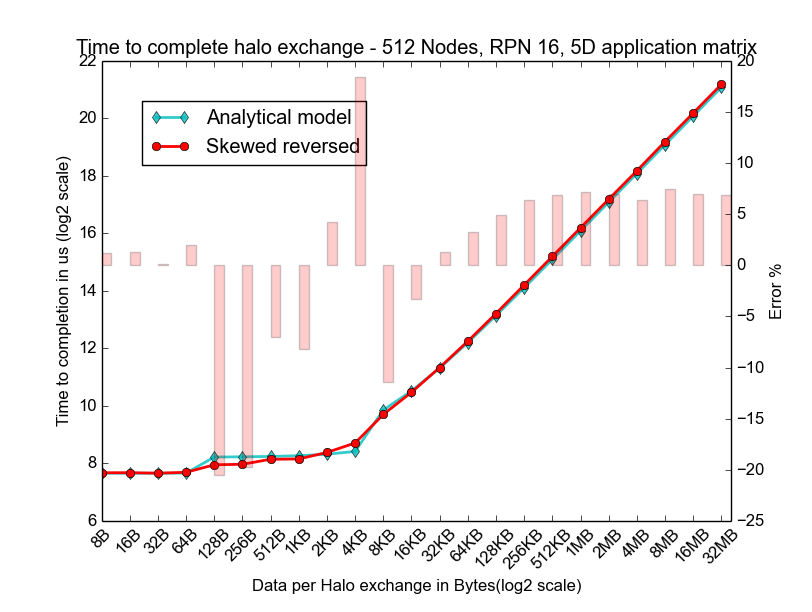
\includegraphics[width=1\textwidth]{../mappings/3d_skewed_reversed.png}
  \end{column}
  \begin{column}{0.3\textwidth}
\lstset{title=Mapping sample}
\begin{lstlisting}[basicstyle=\footnotesize\ttfamily, frame=lines,columns=fixed]
0 0 0 0 0 0
2 0 0 0 0 0
1 0 0 0 0 0
3 0 0 0 0 0
0 2 0 0 0 0
2 2 0 0 0 0
1 2 0 0 0 0
3 2 0 0 0 0
\end{lstlisting}
  \end{column}
\end{columns}
\end{figure}
\end{frame}
%------------------------------------------------

%------------------------------------------------
\begin{frame}
\begin{figure}
\caption{3D Random mapping}
    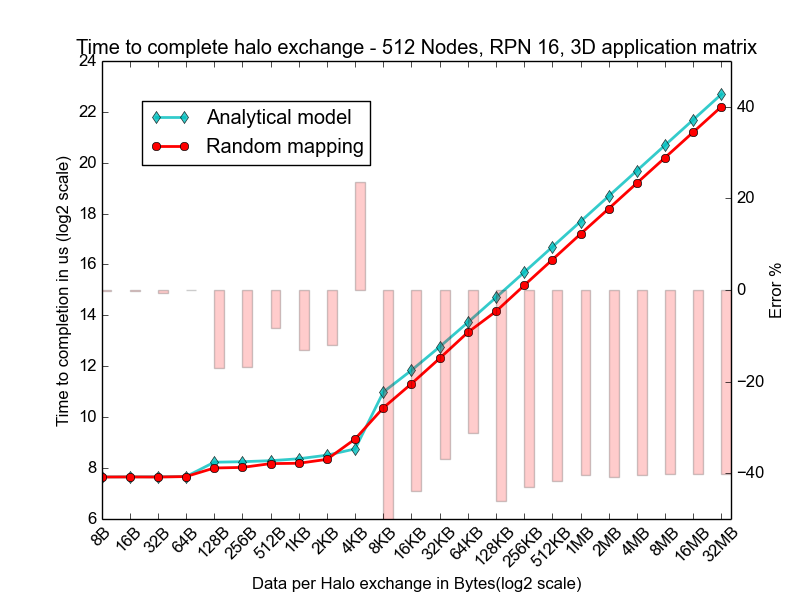
\includegraphics[width=0.75\textwidth]{../mappings/3d_random.png}
\end{figure}
\end{frame}
%------------------------------------------------

%------------------------------------------------
\begin{frame}[fragile]
\begin{figure}
\caption{3D Optimal mapping}
\begin{columns}
  \begin{column}{0.6\textwidth}
    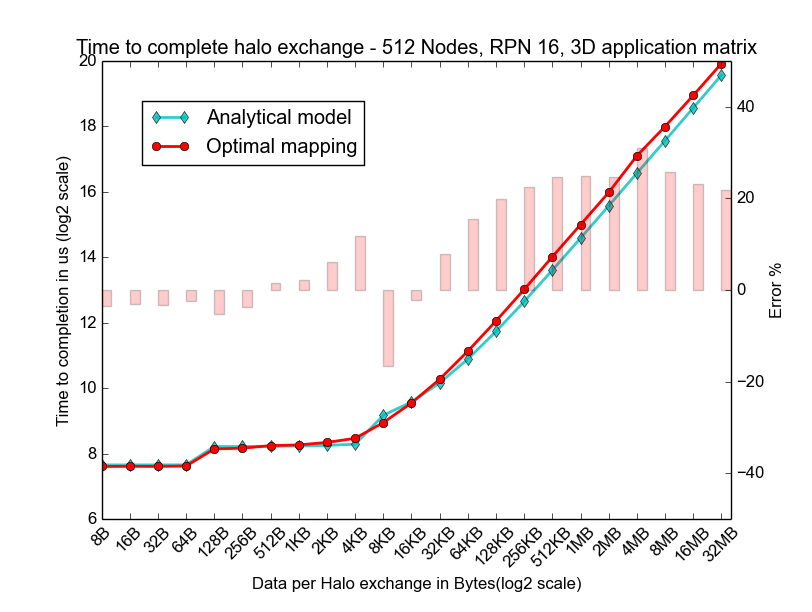
\includegraphics[width=1\textwidth]{../mappings/3d_optimal.png}
  \end{column}
  \begin{column}{0.3\textwidth}
\lstset{title=Mapping sample}
\begin{lstlisting}[basicstyle=\footnotesize\ttfamily, frame=lines,columns=fixed]
0 0 0 0 0 0
0 0 0 0 0 1
0 0 1 0 0 0
0 0 1 0 0 1
0 0 2 0 0 0
0 0 2 0 0 1
0 0 3 0 0 0
0 0 3 0 0 1
\end{lstlisting}
  \end{column}
\end{columns}
\end{figure}
\end{frame}
%------------------------------------------------

%------------------------------------------------
\begin{frame}[fragile]
\begin{figure}
\caption{3D Pessimal mapping}
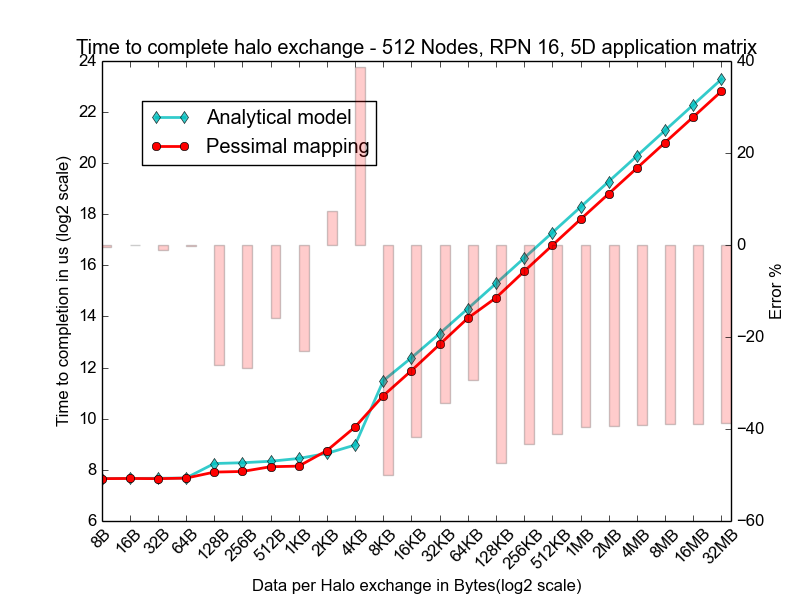
\includegraphics[width=0.75\textwidth]{../mappings/3d_pessimal.png}
\end{figure}
\end{frame}
%------------------------------------------------


%------------------------------------------------
\begin{frame}[fragile]
\begin{figure}
\caption{Analytical model effectiveness}
\begin{table}
  \caption{3D Experimental data vs Analytical model
    \label{table:data vs model 3d}}
  {\footnotesize
    \begin{tabular}{ | l | l | l | p{1.5cm} |}
    \hline
    Mapping    &    Min Error\% &    Max Error\% & Avg abs Error\%\\ \hline
    Optimal    &         -16.63 &          30.88 &         13.17\\ \hline
    Regular    &          -0.49 &          36.68 &         15.31\\ \hline
    Linear     &         -24.12 &          14.00 &         10.91\\ \hline
    Reversed   &         -24.13 &          13.93 &         11.00\\ \hline
    Skewed regular &      -0.39 &          39.57 &         19.81\\ \hline
    Skewed reversed&     -20.52 &          18.44 &          7.04\\ \hline
    Random  &            -53.60 &          23.63 &         27.41\\ \hline
    Pessimal &           -50.07 &          38.67 &         28.79\\ \hline
    \hline
    \end{tabular}
  }
\end{table}
\end{figure}
\end{frame}
%------------------------------------------------

\begin{frame}[fragile]
\begin{figure}
\caption{Analytical model effectiveness}
\begin{table}
  \caption{5D Experimental data vs Analytical model
    \label{table:data vs model 5d}}
  {\footnotesize
    \begin{tabular}{ | l | l | l | p{1.5cm} |}
    \hline
    Mapping         &    Min Error\% &   Max Error\% & Avg abs Error\%\\ \hline
    Optimal         &         -44.12 & 16.01 & 15.88\\ \hline
    Regular         &         -0.41  & 32.42 & 17.07\\ \hline
    Skewed regular  &         -0.68  & 30.98 & 16.96\\ \hline
    Skewed reversed &         -9.31  & 17.69 & 8.99\\ \hline
    Linear          &         -9.44  & 17.20 & 6.71\\ \hline
    Reversed        &         -9.36  & 17.12 & 6.64\\ \hline
    Random          &         -35.86 & 35.19 & 15.69\\ \hline

    \hline
    \end{tabular}
  }
\end{table}

\end{figure}
\end{frame}
%------------------------------------------------



\end{document} 
